% Created 2026-04-16 Thu 23:40
% Intended LaTeX compiler: pdflatex
\documentclass{article}
\usepackage[utf8]{inputenc}
\usepackage[T1]{fontenc}
\usepackage{graphicx}
\usepackage{longtable}
\usepackage{wrapfig}
\usepackage{rotating}
\usepackage[normalem]{ulem}
\usepackage{amsmath}
\usepackage{amssymb}
\usepackage{capt-of}
\usepackage{hyperref}

\usepackage{fancyhdr}
\usepackage[top=25mm, left=25mm, right=25mm]{geometry}
\usepackage{longtable}
\fancyhead[R]{}
\setlength\headheight{43.0pt}
\usepackage{tabularx}
\usepackage{longtable}
\author{Alban Salazar Emilio Fabian, Auz Montezuma Juan Diego , Luisa Calapiña Henry Paul, Quillupangui Lozano Ana María}
\date{2026-04-08}
\title{Taller de Configuración de Entorno WSL}
\hypersetup{
 pdfauthor={Alban Salazar Emilio Fabian, Auz Montezuma Juan Diego , Luisa Calapiña Henry Paul, Quillupangui Lozano Ana María},
 pdftitle={Taller de Configuración de Entorno WSL},
 pdfkeywords={},
 pdfsubject={},
 pdfcreator={Emacs 27.1 (Org mode 9.7.5)}, 
 pdflang={Espanol}}
\begin{document}

\maketitle
\fancyhead[C]{\includegraphics[scale=0.05]{../images/logoEPN.jpg}\\
ESCUELA POLITECNICA NACIONAL\\FACULTAD DE INGENIERIA DE SISTEMAS\\
ARQUITECTURA DE COMPUTADORES}
\thispagestyle{fancy}

\section{Objetivos}
\label{sec:orgaf14a44}

\begin{itemize}
\item Configurar y validar el entorno de trabajo para la asignatura de Arquitectura de Computadores en Linux o WSL.
\item Verificar la instalación de herramientas base: mamba/anaconda (Python), Emacs y \LaTeX.
\item Documentar evidencias técnicas mediante capturas y comandos ejecutados.
\end{itemize}

\section{Instrucciones}
\label{sec:orgfb1f43d}

\begin{enumerate}
\item Realice todas las actividades en Linux o en WSL.
\item En cada sección ejecute los comandos solicitados y registre la salida en el bloque correspondiente.
\item Guarde el archivo y exporte a pdf con el comando `org-latex-export-to-pdf`.
\item Verifique que estén todos los nombres de los integrantes del grupo
de trabajo. Los grupos para este trabajo están en \href{https://epnecuador.sharepoint.com/:x:/s/ICCD332-ArquitecturaComputadores/IQCjNuELSDbJTb42EfrLL2ksATBSbitbZ9\_iFLJxIiCtSr0?e=gowv5I}{Equipos de Trabajo}.
\item Verifique que en las distintas secciones de este archivo esté
identificado con nombre e email el aporte del estudiante.
\end{enumerate}

Si requiere insertar una imagen, crear una carpeta \texttt{images} y colocar
la imagen dentro. Para llamar la imagen desde Emacs use \texttt{C-c C-l} y
busque el archivo o escriba:Puede insertar una imagen con la sintaxis:

\begin{verbatim}
[[./images/image1.jpg]]
\end{verbatim}
\section{Actividades}
\label{sec:org48f14ec}
\subsection{Configuración de WSL con Ubuntu, \LaTeX, Python e Emacs}
\label{sec:orge2d1c62}

\begin{enumerate}
\item Verificación de entorno mamba/anaconda
\begin{enumerate}
\item Active WSL (si aplica) y su entorno de trabajo.
\item Ejecute \texttt{mamba info} con \texttt{C-c C-c} dentro del bloque de código.
\item Si el comando falla, active un entorno con \texttt{mamba activate iccd332} e intente de nuevo.
\end{enumerate}
\end{enumerate}
\subsubsection{Estudiante A: Alban Salazar Emilio Fabian}
\label{sec:org5696e2e}
\begin{verbatim}
  mamba info
\end{verbatim}
\begin{verbatim}

       libmamba version : 2.5.0
          mamba version : 2.5.0
           curl version : libcurl/8.19.0 OpenSSL/3.6.1 zlib/1.3.2 zstd/1.5.7 libssh2/1.11.1 nghttp2/1.68.1 mit-krb5/1.22.2
     libarchive version : libarchive 3.8.6 zlib/1.3.2 liblzma/5.8.2 bz2lib/1.0.8 liblz4/1.10.0 libzstd/1.5.7 liblzo2/2.10 openssl/3.5.5 libb2/bundled
       envs directories : /home/emilioalbanfs/miniforge3/envs
          package cache : /home/emilioalbanfs/miniforge3/pkgs
                          /home/emilioalbanfs/.mamba/pkgs
            environment : iccd332 (active)
           env location : /home/emilioalbanfs/miniforge3/envs/iccd332
      user config files : /home/emilioalbanfs/.mambarc
 populated config files : /home/emilioalbanfs/miniforge3/.condarc
       virtual packages : __unix=0=0
                          __linux=6.6.87=0
                          __glibc=2.39=0
                          __archspec=1=x86_64_v3
               channels : https://conda.anaconda.org/conda-forge/linux-64
                          https://conda.anaconda.org/conda-forge/noarch
       base environment : /home/emilioalbanfs/miniforge3
               platform : linux-64
\end{verbatim}
\subsubsection{Estudiante B: Auz Montezuma Juan Diego}
\label{sec:org98cc879}
\begin{verbatim}
  mamba info
\end{verbatim}
\begin{verbatim}

       libmamba version : 2.5.0
          mamba version : 2.5.0
           curl version : libcurl/8.19.0 OpenSSL/3.6.1 zlib/1.3.2 zstd/1.5.7 libssh2/1.11.1 nghttp2/1.68.1 mit-krb5/1.22.2
     libarchive version : libarchive 3.8.6 zlib/1.3.2 liblzma/5.8.2 bz2lib/1.0.8 liblz4/1.10.0 libzstd/1.5.7 liblzo2/2.10 openssl/3.5.5 libb2/bundled
       envs directories : /home/juand/miniforge3/envs
          package cache : /home/juand/miniforge3/pkgs
                          /home/juand/.mamba/pkgs
            environment : iccd332 (active)
           env location : /home/juand/miniforge3/envs/iccd332
      user config files : /home/juand/.mambarc
 populated config files : /home/juand/miniforge3/.condarc
       virtual packages : __unix=0=0
                          __linux=6.18.2=0
                          __glibc=2.42=0
                          __archspec=1=x86_64_v3
               channels : https://conda.anaconda.org/conda-forge/linux-64
                          https://conda.anaconda.org/conda-forge/noarch
       base environment : /home/juand/miniforge3
               platform : linux-64
\end{verbatim}
\subsubsection{Estudiante C: Henry Luisa}
\label{sec:org33c280f}
\begin{verbatim}
  mamba info
\end{verbatim}
\begin{verbatim}

       libmamba version : 2.5.0
          mamba version : 2.5.0
           curl version : libcurl/8.19.0 OpenSSL/3.6.1 zlib/1.3.2 zstd/1.5.7 libssh2/1.11.1 nghttp2/1.68.1 mit-krb5/1.22.2
     libarchive version : libarchive 3.8.6 zlib/1.3.2 liblzma/5.8.2 bz2lib/1.0.8 liblz4/1.10.0 libzstd/1.5.7 liblzo2/2.10 openssl/3.5.5 libb2/bundled
       envs directories : /home/emilioalbanfs/miniforge3/envs
          package cache : /home/emilioalbanfs/miniforge3/pkgs
                          /home/emilioalbanfs/.mamba/pkgs
            environment : iccd332 (active)
           env location : /home/emilioalbanfs/miniforge3/envs/iccd332
      user config files : /home/emilioalbanfs/.mambarc
 populated config files : /home/emilioalbanfs/miniforge3/.condarc
       virtual packages : __unix=0=0
                          __linux=6.6.87=0
                          __glibc=2.39=0
                          __archspec=1=x86_64_v3
               channels : https://conda.anaconda.org/conda-forge/linux-64
                          https://conda.anaconda.org/conda-forge/noarch
       base environment : /home/emilioalbanfs/miniforge3
               platform : linux-64
\end{verbatim}

\subsubsection{Estudiante D: Quillupangui Lozano Ana Maria}
\label{sec:org8d7c12d}
\begin{verbatim}
  mamba info
\end{verbatim}
\begin{verbatim}

       libmamba version : 2.5.0
          mamba version : 2.5.0
           curl version : libcurl/8.19.0 OpenSSL/3.6.1 zlib/1.3.2 zstd/1.5.7 libssh2/1.11.1 nghttp2/1.68.1 mit-krb5/1.22.2
     libarchive version : libarchive 3.8.6 zlib/1.3.2 liblzma/5.8.2 bz2lib/1.0.8 liblz4/1.10.0 libzstd/1.5.7 liblzo2/2.10 openssl/3.5.5 libb2/bundled
       envs directories : /home/emilioalbanfs/miniforge3/envs
          package cache : /home/emilioalbanfs/miniforge3/pkgs
                          /home/emilioalbanfs/.mamba/pkgs
            environment : iccd332 (active)
           env location : /home/emilioalbanfs/miniforge3/envs/iccd332
      user config files : /home/emilioalbanfs/.mambarc
 populated config files : /home/emilioalbanfs/miniforge3/.condarc
       virtual packages : __unix=0=0
                          __linux=6.6.87=0
                          __glibc=2.39=0
                          __archspec=1=x86_64_v3
               channels : https://conda.anaconda.org/conda-forge/linux-64
                          https://conda.anaconda.org/conda-forge/noarch
       base environment : /home/emilioalbanfs/miniforge3
               platform : linux-64
\end{verbatim}
\subsubsection{Estudiante A: Alban Salazar Emilio Fabian}
\label{sec:org6a1a053}
\begin{verbatim}
    python --version
\end{verbatim}
\begin{verbatim}
Python 3.14.4
\end{verbatim}
\subsubsection{Estudiante B: Auz Montezuma Juan Diego}
\label{sec:orgd1c3189}
\begin{verbatim}
    python --version
\end{verbatim}
\begin{verbatim}
Python 3.11.15
\end{verbatim}
\subsubsection{Estudiante C: Henry Luisa}
\label{sec:orgad46ddb}
\begin{verbatim}
    python --version
\end{verbatim}
\begin{verbatim}
Python 3.14.4
\end{verbatim}
\subsubsection{Estudiante D:Quillupangui Lozano Ana María}
\label{sec:org273345d}
\begin{verbatim}
    python --version 
\end{verbatim}
\begin{verbatim}
Python 3.14.4
\end{verbatim}


\begin{enumerate}
\item Verificacion de Emacs
Ejecute \texttt{emacs -{}-{}version} en la consola y desde Emacs.
\end{enumerate}
\subsubsection{Estudiante A: Alban Salazar Emilio Fabian}
\label{sec:orgd8cb058}
\begin{verbatim}
   emacs --version
\end{verbatim}
\begin{verbatim}
GNU Emacs 29.3
Copyright (C) 2024 Free Software Foundation, Inc.
GNU Emacs comes with ABSOLUTELY NO WARRANTY.
You may redistribute copies of GNU Emacs
under the terms of the GNU General Public License.
For more information about these matters, see the file named COPYING.
\end{verbatim}
\subsubsection{Estudiante B: Auz Montezuma Juan Diego}
\label{sec:org9dbfdac}
\begin{verbatim}
   emacs --version
\end{verbatim}
\begin{verbatim}
GNU Emacs 30.2
Copyright (C) 2025 Free Software Foundation, Inc.
GNU Emacs comes with ABSOLUTELY NO WARRANTY.
You may redistribute copies of GNU Emacs
under the terms of the GNU General Public License.
For more information about these matters, see the file named COPYING.
\end{verbatim}
\subsubsection{Estudiante C: Henry Luisa}
\label{sec:org5ffeafd}
\begin{verbatim}
   emacs --version
\end{verbatim}
\begin{verbatim}
GNU Emacs 29.3
Copyright (C) 2024 Free Software Foundation, Inc.
GNU Emacs comes with ABSOLUTELY NO WARRANTY.
You may redistribute copies of GNU Emacs
under the terms of the GNU General Public License.
For more information about these matters, see the file named COPYING.
\end{verbatim}

\subsubsection{Estudiante D: Quillpangui Lozano Ana María}
\label{sec:org365b063}
\begin{verbatim}
   emacs --version 
\end{verbatim}
\begin{verbatim}
GNU Emacs 29.3
Copyright (C) 2024 Free Software Foundation, Inc.
GNU Emacs comes with ABSOLUTELY NO WARRANTY.
You may redistribute copies of GNU Emacs
under the terms of the GNU General Public License.
For more information about these matters, see the file named COPYING.
\end{verbatim}


\begin{enumerate}
\item Verificacion de \LaTeX{}
Ejecute \texttt{latex -{}-{}version} en la consola y desde Emacs.
\end{enumerate}
\subsubsection{Estudiante A: Alban Salazar Emilio Fabian}
\label{sec:orgdab2276}
\begin{verbatim}
   latex --version
\end{verbatim}
\begin{verbatim}
   pdfTeX 3.141592653-2.6-1.40.25 (TeX Live 2023/Debian)
   kpathsea version 6.3.5
   Copyright 2023 Han The Thanh (pdfTeX) et al.
   There is NO warranty.  Redistribution of this software is
   covered by the terms of both the pdfTeX copyright and
   the Lesser GNU General Public License.
   For more information about these matters, see the file
   named COPYING and the pdfTeX source.
   Primary author of pdfTeX: Han The Thanh (pdfTeX) et al.
   Compiled with libpng 1.6.43; using libpng 1.6.43
   Compiled with zlib 1.3; using zlib 1.3
   Compiled with xpdf version 4.04
\end{verbatim}
\subsubsection{Estudiante B: Auz Montezuma Juan Diego}
\label{sec:org957dace}
\begin{verbatim}
   latex --version
\end{verbatim}
\begin{verbatim}
   pdfTeX 3.141592653-2.6-1.40.27 (TeX Live 2026/dev/Arch Linux)
   kpathsea version 6.4.2/dev
   Copyright 2025 Han The Thanh (pdfTeX) et al.
   There is NO warranty.  Redistribution of this software is
   covered by the terms of both the pdfTeX copyright and
   the Lesser GNU General Public License.
   For more information about these matters, see the file
   named COPYING and the pdfTeX source.
   Primary author of pdfTeX: Han The Thanh (pdfTeX) et al.
   Compiled with libpng 1.6.50; using libpng 1.6.53
   Compiled with zlib 1.3.1; using zlib 1.3.1
   Compiled with xpdf version 4.04
\end{verbatim}
\subsubsection{Estudiante C: Henry Luisa}
\label{sec:org76c5a58}
\begin{verbatim}
   latex --version
\end{verbatim}
\begin{verbatim}
   pdfTeX 3.141592653-2.6-1.40.25 (TeX Live 2023/Debian)
   kpathsea version 6.3.5
   Copyright 2023 Han The Thanh (pdfTeX) et al.
   There is NO warranty.  Redistribution of this software is
   covered by the terms of both the pdfTeX copyright and
   the Lesser GNU General Public License.
   For more information about these matters, see the file
   named COPYING and the pdfTeX source.
   Primary author of pdfTeX: Han The Thanh (pdfTeX) et al.
   Compiled with libpng 1.6.43; using libpng 1.6.43
   Compiled with zlib 1.3; using zlib 1.3
   Compiled with xpdf version 4.04
\end{verbatim}
\subsubsection{Estudiante D:Quillpangui Lozano Ana María}
\label{sec:org7ac358c}
\begin{verbatim}
   latex --version 
\end{verbatim}
\begin{verbatim}
   pdfTeX 3.141592653-2.6-1.40.25 (TeX Live 2023/Debian)
   kpathsea version 6.3.5
   Copyright 2023 Han The Thanh (pdfTeX) et al.
   There is NO warranty.  Redistribution of this software is
   covered by the terms of both the pdfTeX copyright and
   the Lesser GNU General Public License.
   For more information about these matters, see the file
   named COPYING and the pdfTeX source.
   Primary author of pdfTeX: Han The Thanh (pdfTeX) et al.
   Compiled with libpng 1.6.43; using libpng 1.6.43
   Compiled with zlib 1.3; using zlib 1.3
   Compiled with xpdf version 4.04
\end{verbatim}

\begin{enumerate}
\item Registro de problemas y solución aplicada
\end{enumerate}

Complete la siguiente tabla si tuvo errores durante la configuración:

\begin{center}
\begin{tabularx}{\textwidth}{lXX}
\textbf{Herramienta} & \textbf{Problema observado} & \textbf{Solución aplicada}\\[0pt]
\hline
 &  & \\[0pt]
 &  & \\[0pt]
 &  & \\[0pt]
\end{tabularx}
\end{center}

\subsection{Comandos Emacs Tutorial}
\label{sec:org5a71b1c}
Seguir el tutorial integrado en Emacs al respecto de la navegación y
operaciones más frecuentes. El tutorial puede ser accedido en Español
utilizando el comando:

\begin{verbatim}
M-x help-with-tutorial-spec-language
\end{verbatim}

Realice los ejercicios del tutorial (al menos un 80\% del texto) y
complete la siguiente tabla con los comandos que considere de mayor
interés. Verifique que en la parte superior se active el menú de
tabla. Dentro de la región de la tabla puede dar C-c C-c para alinear
automáticamente la tabla al contenido del texto que escriba. Para
generar una nueva fila escriba presione la tecla TAB

<Estudiante A> Alban Salazar Emilio Fabian
\begin{longtable}{|p{0.2\linewidth}|p{0.3\linewidth}|p{0.2\linewidth}|p{0.3\linewidth}|}
\textbf{Comando} & \textbf{Descripción} & \textbf{Comando} & \textbf{Descripción}\\[0pt]
\hline
\endfirsthead
\multicolumn{4}{l}{Continued from previous page} \\[0pt]
\hline

\textbf{Comando} & \textbf{Descripción} & \textbf{Comando} & \textbf{Descripción} \\[0pt]

\hline
\endhead
\hline\multicolumn{4}{r}{Continued on next page} \\
\endfoot
\endlastfoot
\hline
\texttt{C-g} & Cancelar un comando parcialmente introducido & \texttt{M-b / M-f} & Moverse atrás/adelante de una palabra\\[0pt]
\texttt{C-k} & Elimina desde el cursor hasta el fin de la línea & \texttt{M-w} & Copiar un segmento de texto\\[0pt]
\texttt{C-<SPC>} & Resaltar un texto entre el cursos y la posición en la que se tecleó & \texttt{C-/} & Para deshacer cambios\\[0pt]
\end{longtable}

<Estudiante B> Auz Montezuma Juan Diego
\begin{longtable}{|p{0.2\linewidth}|p{0.3\linewidth}|p{0.2\linewidth}|p{0.3\linewidth}|}
\textbf{Comando} & \textbf{Descripción} & \textbf{Comando} & \textbf{Descripción}\\[0pt]
\hline
\endfirsthead
\multicolumn{4}{l}{Continued from previous page} \\[0pt]
\hline

\textbf{Comando} & \textbf{Descripción} & \textbf{Comando} & \textbf{Descripción} \\[0pt]

\hline
\endhead
\hline\multicolumn{4}{r}{Continued on next page} \\
\endfoot
\endlastfoot
\hline
\texttt{C-x C-f} & Abrir/Guardar archivos & \texttt{C-x 1} & Centrar la pantalla en un solo buffer\\[0pt]
\texttt{C-a / C-e} & Moverse al inicio o final de la oración & \texttt{C-space M-w} & Copiar el texto seleccionado\\[0pt]
\texttt{C-y} & Pegar & \texttt{C-/ o C-x u} & Revertir cambios\\[0pt]
\end{longtable}

<Estudiante C> Henry Luisa
\begin{longtable}{|p{0.2\linewidth}|p{0.3\linewidth}|p{0.2\linewidth}|p{0.3\linewidth}|}
\textbf{Comando} & \textbf{Descripción} & \textbf{Comando} & \textbf{Descripción}\\[0pt]
\hline
\endfirsthead
\multicolumn{4}{l}{Continued from previous page} \\[0pt]
\hline

\textbf{Comando} & \textbf{Descripción} & \textbf{Comando} & \textbf{Descripción} \\[0pt]

\hline
\endhead
\hline\multicolumn{4}{r}{Continued on next page} \\
\endfoot
\endlastfoot
\hline
\texttt{C-x b} & Cambiar entre buffers & \texttt{M-v} & Desplazarse hacia arriba\\[0pt]
\texttt{C-g} & Cancela un comando en ejecución & \texttt{C-k} & Borra la linea\\[0pt]
\texttt{C-l} & Refrescar y centrar la pantalla & \texttt{C-w} & Corta el contenido seleccionado\\[0pt]
\end{longtable}

<Estudiante D> Quillupangui Lozano Ana María
\begin{longtable}{|p{0.2\linewidth}|p{0.3\linewidth}|p{0.2\linewidth}|p{0.3\linewidth}|}
\textbf{Comando} & \textbf{Descripción} & \textbf{Comando} & \textbf{Descripción}\\[0pt]
\hline
\endfirsthead
\multicolumn{4}{l}{Continued from previous page} \\[0pt]
\hline

\textbf{Comando} & \textbf{Descripción} & \textbf{Comando} & \textbf{Descripción} \\[0pt]

\hline
\endhead
\hline\multicolumn{4}{r}{Continued on next page} \\
\endfoot
\endlastfoot
\hline
\texttt{C-x C-c} & Cerrar Sesión & \texttt{C-c C-c} & Ejecutar acción\\[0pt]
\texttt{M-a / M-e} & Moverse al final/inicio de la oración & \texttt{C-x 2} & Dividir Horizontalmente\\[0pt]
\texttt{C-x 1} & Dejar la ventana principal & \texttt{C-h ?} & Ayuda general\\[0pt]
\end{longtable}
\subsection{Comandos Emacs Juego}
\label{sec:org16b7427}
En la anterior sección usted revisó los comandos de mayor interés
sobre la manipulación de Emacs. Es hora de poner en práctica sus
conocimientos. Realice unas 3 visitas al juego  \href{https://chat.qwen.ai/s/deploy/t\_23ff57ef-b59a-4bd7-9b79-54679b33686d}{Emacs-Trainer} y apunte
en la siguiente tabla su puntaje.

Estudiante A: Alban Salazar Emilio Fabian
\begin{center}
\begin{tabular}{rr}
\hline
iteración & Puntaje\\[0pt]
\hline
1 & 140\\[0pt]
2 & 130\\[0pt]
3 & 140\\[0pt]
\hline
\end{tabular}
\end{center}

\begin{enumerate}
\item Intento 1
\label{sec:orge4eb5dc}
\begin{center}
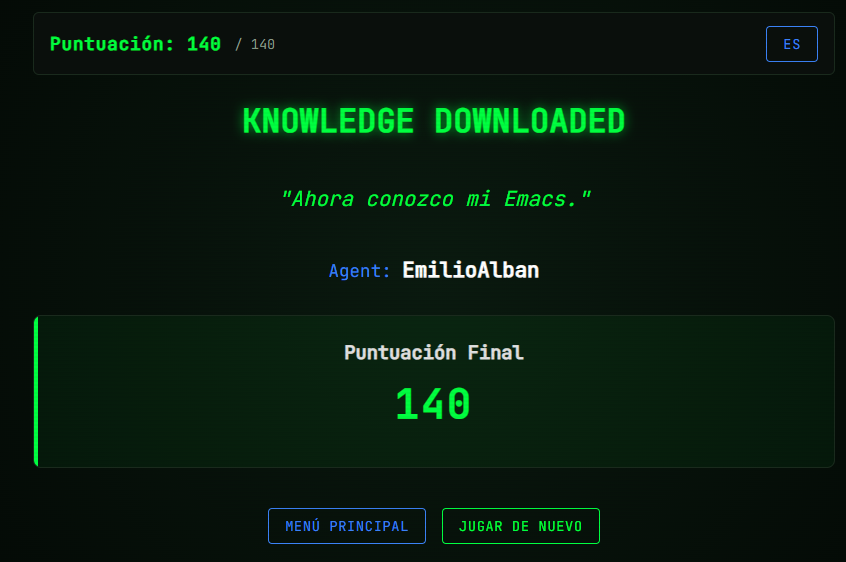
\includegraphics[width=.9\linewidth]{./images/EmilioAlban-1.png}
\end{center}
\item Intento 2
\label{sec:org60c2bde}
\begin{center}
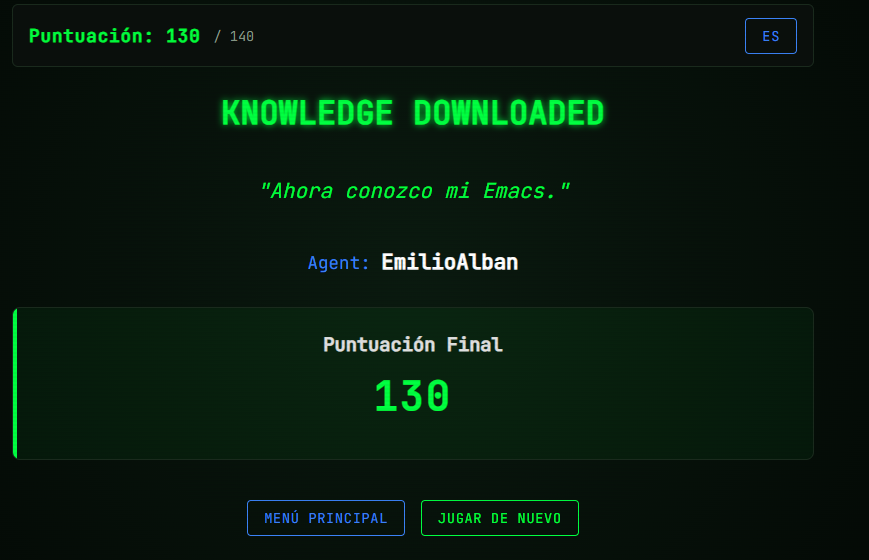
\includegraphics[width=.9\linewidth]{./images/EmilioAlban-2.png}
\end{center}
\item Intento 3
\label{sec:org7608441}
\begin{center}
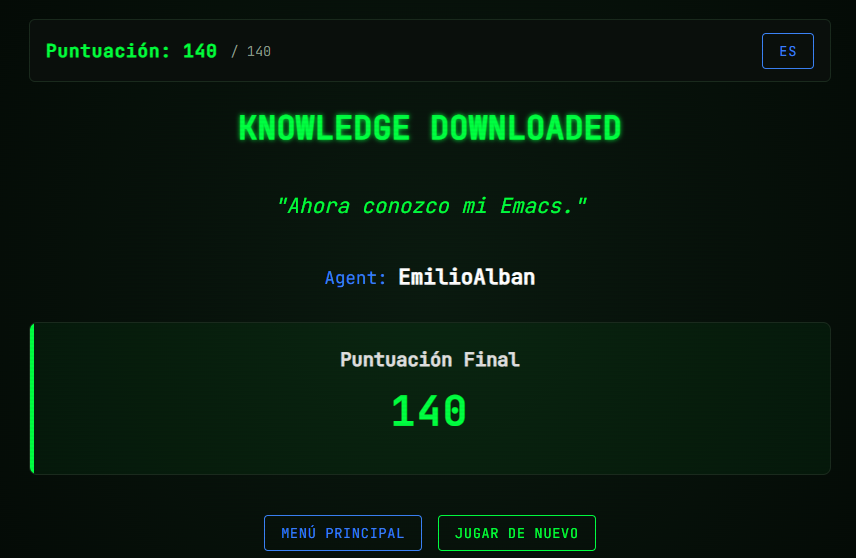
\includegraphics[width=.9\linewidth]{./images/EmilioAlban-3.png}
\end{center}

Estudiante B: Auz Montezuma Juan Diego 
\begin{center}
\begin{tabular}{rr}
\hline
iteración & Puntaje\\[0pt]
\hline
1 & 140\\[0pt]
2 & 140\\[0pt]
3 & 140\\[0pt]
\hline
\end{tabular}
\end{center}

\item Intento 1
\label{sec:orgbcedfa4}
\begin{center}
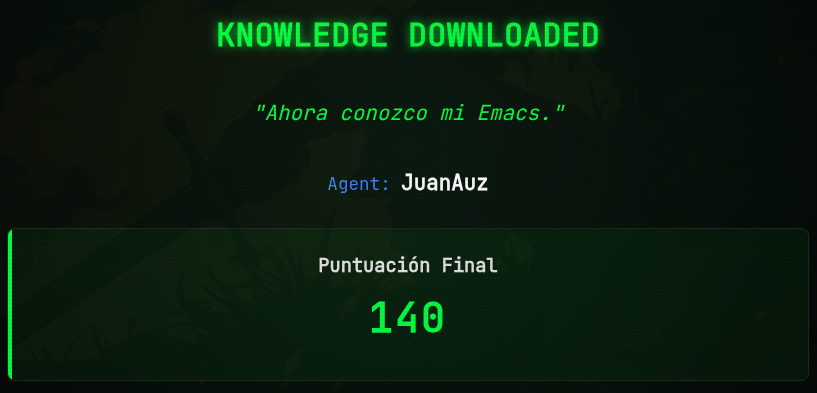
\includegraphics[width=.9\linewidth]{./images/JuanAuz-1.png}
\end{center}
\item Intento 2
\label{sec:org2a19f8f}
\begin{center}

\includegraphics[width=.9\linewidth]{./images/JuanAuz-2.png}
\end{center}
\item Intento 3
\label{sec:org26ad4d5}
\begin{center}
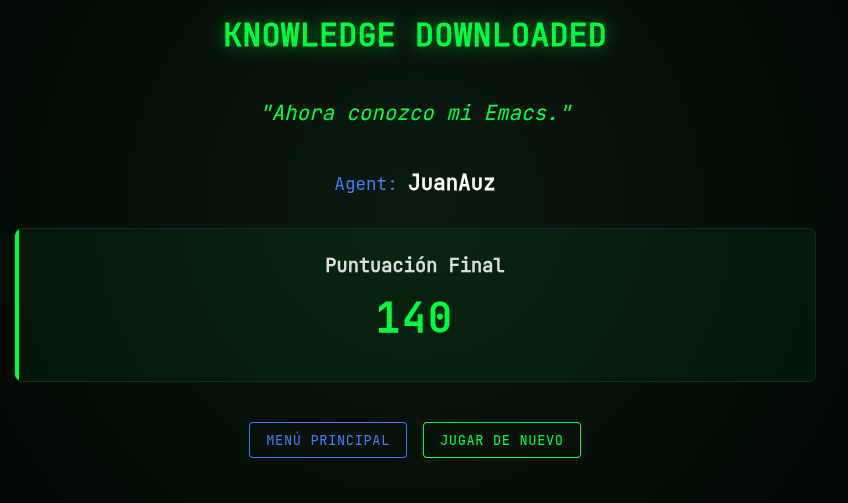
\includegraphics[width=.9\linewidth]{./images/JuanAuz-3.png}
\end{center}
Estudiante C: Henry Luisa 
\begin{center}
\begin{tabular}{rr}
\hline
iteración & Puntaje\\[0pt]
\hline
1 & 134\\[0pt]
2 & 140\\[0pt]
3 & 140\\[0pt]
\hline
\end{tabular}
\end{center}
\item Intento 1
\label{sec:org477c1ad}
\begin{center}
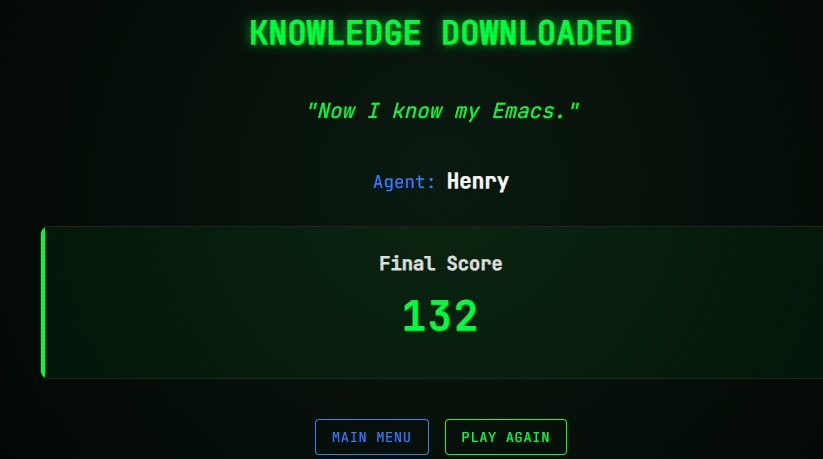
\includegraphics[width=.9\linewidth]{images/Henry-1.jpeg}
\end{center}
\item Intento 2
\label{sec:org97399f5}
\begin{center}
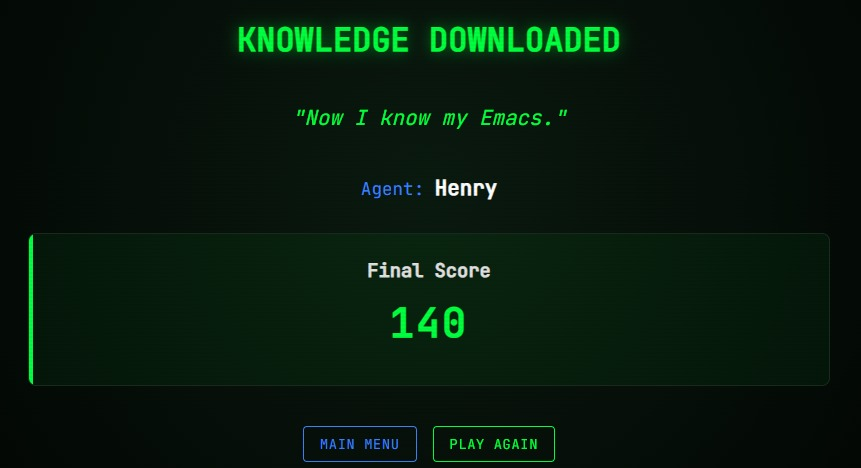
\includegraphics[width=.9\linewidth]{images/Henry-2.jpeg}
\end{center}
\item Intento 3
\label{sec:org19013df}
\begin{center}
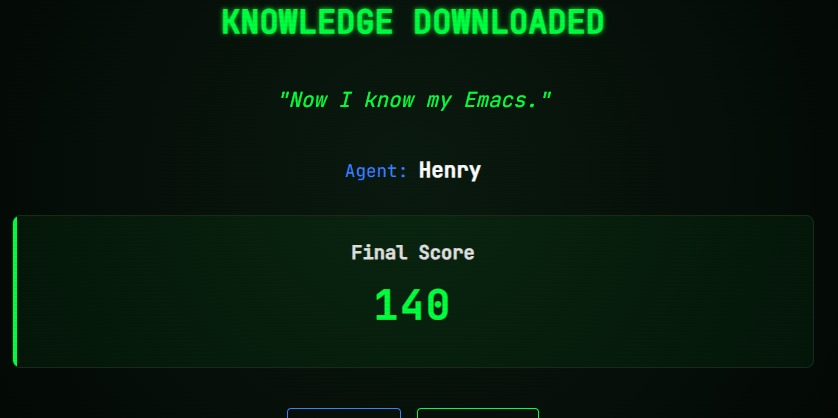
\includegraphics[width=.9\linewidth]{images/Henry-3.jpeg}
\end{center}
\begin{verbatim}
[[./estudianteC-game.png]]
\end{verbatim}

Estudiante D: Quillpangui Lozano Ana María
\begin{center}
\begin{tabular}{rr}
\hline
iteración & Puntaje\\[0pt]
\hline
1 & 64\\[0pt]
2 & 115\\[0pt]
3 & 126\\[0pt]
\hline
\end{tabular}
\end{center}
\item Intento 1
\label{sec:orgb91b6e7}
\begin{center}
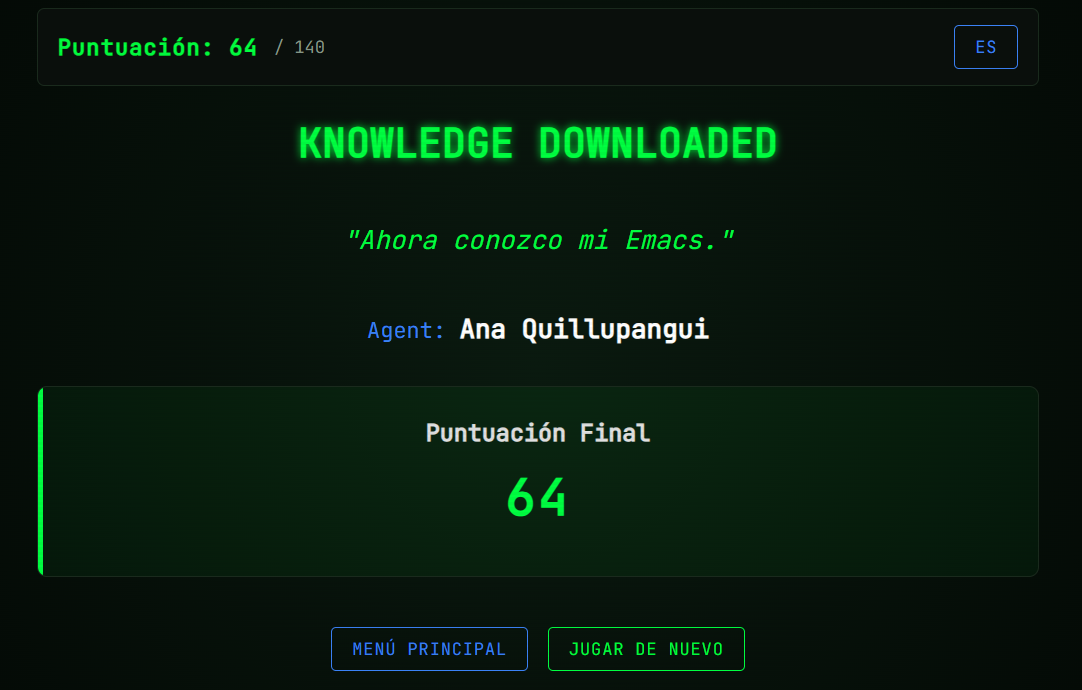
\includegraphics[width=.9\linewidth]{./images/AnaQuillupangui-1.png}
\end{center}

\item Intento 2
\label{sec:org394b6ff}
\begin{center}
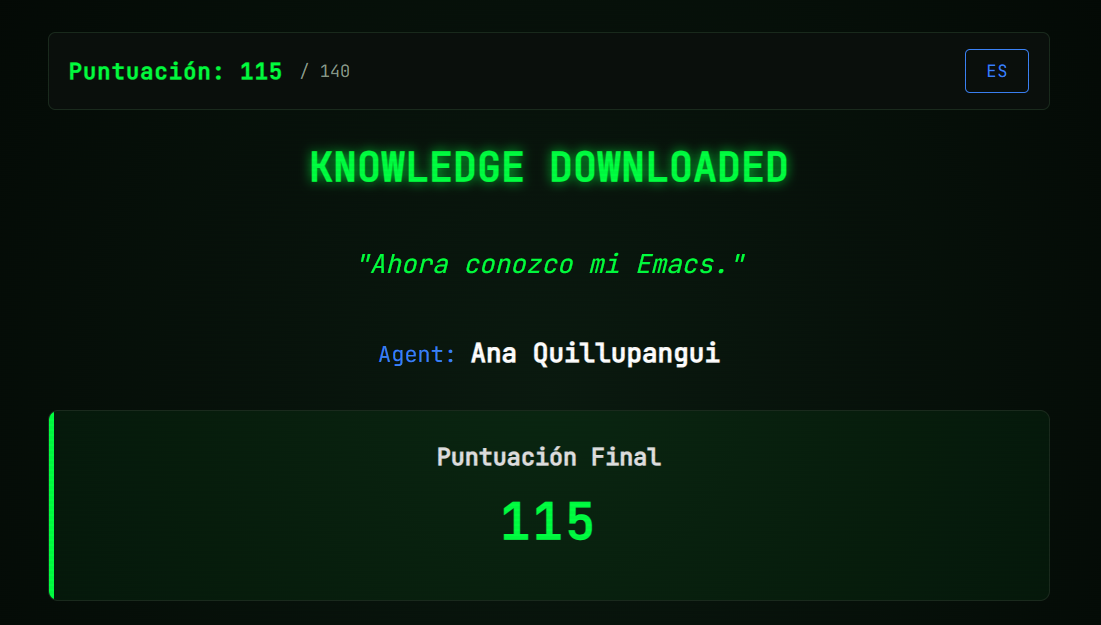
\includegraphics[width=.9\linewidth]{./images/AnaQuillupangui-2.png}
\end{center}
\item Intento 3
\label{sec:org6330cc7}
\begin{center}
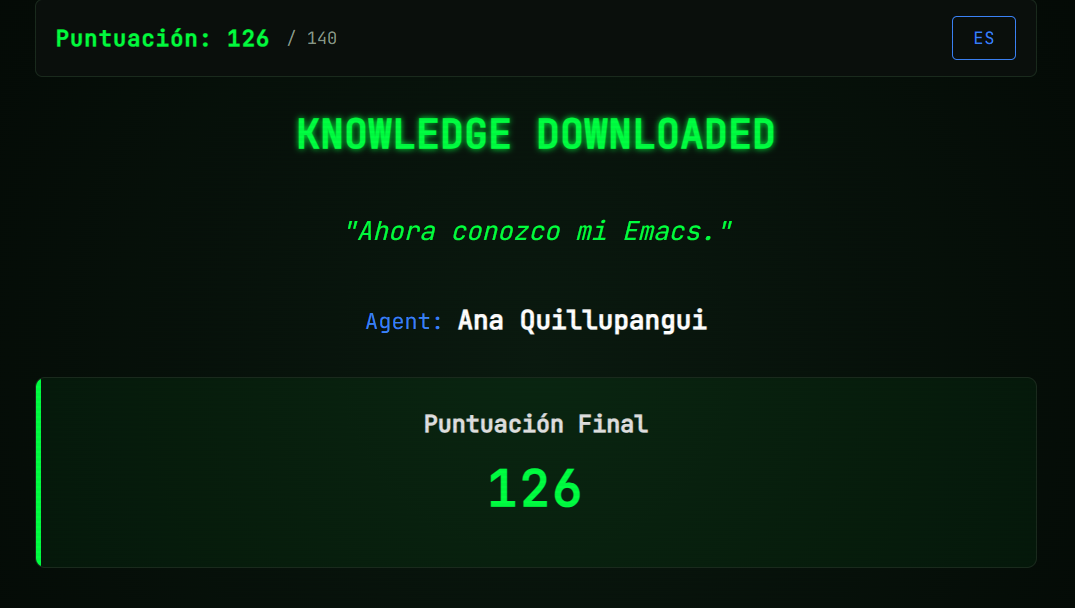
\includegraphics[width=.9\linewidth]{./images/AnaQuillupangui-3.png}
\end{center}
\end{enumerate}

\subsection{}
\label{sec:org56fc366}
\subsection{Usando Emacs para tener Ayuda sobre Emacs}
\label{sec:orgdb215f1}
¿Qué comandos le resultan más fáciles de usar y cuáles le son más
extraños? Identifique 4 comandos que le sean fáciles y 4 que le
resulten complicados. Revise qué dice la ayuda de Emacs sobre cada
comando y escriba en sus palabras el para qué sirve.

Para consultar lo que hace un comando ejecute:
\begin{enumerate}
\item \texttt{C-h k}
\item Emacs le preguntara cuál es la combinación de la que requiere
ayuda. Presione las teclas del comando. Por ejemplo, \texttt{C-x C-f}
\item Emacs abrirá un nuevo buffer con la descripción del comando.
\item Cambie al buffer de la ayuda con \texttt{C-x o}
\item Seleccione el primer párrafo de ayuda ubicando el cursor al inicio
del párrafo y activando la marcación de texto con
\texttt{C-SPC}. Seleccione avanzando por palabras \texttt{M-f} o directamente
toda la linea \texttt{C-e}
\item Una vez seleccionado, copie el texto con \texttt{M-w}.
\item Regrese al buffer anterior con \texttt{C-x o}.
\item Pegue el texto en <Pegar lo que dice el\ldots{}> con \texttt{C-y}
\end{enumerate}

\textbf{\textbf{Comandos Fáciles}}
\begin{enumerate}
\item \textbf{\textbf{Estudiante A: Alban Salazar Emilio Fabian}} \texttt{C-<SPC>} runs the command set-mark-command (found in global-map), which
\end{enumerate}
is an interactive native-compiled Lisp function in ‘simple.el’. El 
comando resalta un texto entre el cursor y la posicion en la que se tecleó
\begin{enumerate}
\item \textbf{\textbf{Estudiante B: Auz Montezuma Juan Diego}} \texttt{C-/}. C-/ runs the command undo (found in global-map), which is an
\end{enumerate}
interactive native-comp-function in ‘simple.el’. El comando deshace el
último (o últimos) cambios que fueron realizados
\begin{enumerate}
\item \textbf{\textbf{Estudiante C: Henry Luisa}} \textasciitilde{}C-v\textasciitilde{}C-v runs the command
\end{enumerate}
scroll-up-command (found in global-map), which is an interactive
native-compiled Lisp function in ‘window.el’.   
\begin{enumerate}
\item \textbf{\textbf{Estudiante D: Quillupangui Lozano Ana María}} \texttt{C-x C-f} <C-x C-f runs the command find-file (found in global-map), which is an
\end{enumerate}
interactive native-compiled Lisp function in ‘files.el’.>El comando
permite abrir o crear un nuevo documento

\textbf{\textbf{Comandos Difíciles}}
\begin{enumerate}
\item \textbf{\textbf{Estudiante A: Alban Salazar Emilio Fabian}} \texttt{C-h c} runs the command describe-key-briefly (found in global-map),
\end{enumerate}
which is an interactive native-compiled Lisp function in ‘help.el’. El
comando permite presionar cualquier otra combinación de teclas para averiguar qué función o comando de Emacs está asignado a ella.
\begin{enumerate}
\item \textbf{\textbf{Estudiante B:Auz Montezuma Juan Diego}} \texttt{C-x b}. C-x b runs the command switch-to-buffer (found in global-map), which
\end{enumerate}
is an interactive native-comp-function in ‘window.el’. El comando abre
el menú para cambiar de un buffer a otro
\begin{enumerate}
\item \textbf{\textbf{Estudiante C: Henry Luisa}} \texttt{C-c C-l} C-x C-l runs the command
downcase-region (found in global-map), which is an interactive
built-in function in ‘C source code’.
\item \textbf{\textbf{Estudiante D:Quillupangui Lozano Ana María}} \texttt{C-s}. <C-s runs the command isearch-forward (found in global-map), which is
\end{enumerate}
an interactive native-compiled Lisp function in ‘isearch.el’.>Permite
buscar texto en el archivo 

\section{Equipo de Trabajo}
\label{sec:orgfb5f46a}
Complete la información de los integrantes de grupo e indique el líder
de grupo.

\begin{center}
\begin{tabular}{lll}
\hline
Nombre & email & Rol\\[0pt]
\hline
Auz Montezuma Juan Diego & juan.auzmontezuma@epn.edu.ec & líder\\[0pt]
Luisa Calapiña Henry Paul & henry.luisa@epn.edu.ec & colaborador\\[0pt]
Quillpangui Lozano Ana María & anamaria.quillpangui@epn.edu.ec & colaborador\\[0pt]
Alban Salazar Emilio Fabian & emilio.alban@epn.edu.ec & colaborador\\[0pt]
 &  & \\[0pt]
\hline
\end{tabular}
\end{center}

\section{Verificación de Entregables [100\%]:}
\label{sec:orgda56fbb}
Ejecute \texttt{C-c C-c} sobre los ítems de tarea según se hayan cumplido o
no. Si un ítem no pudo realizarse apunte en la siguiente sección las
razones al respecto.
\begin{itemize}
\item[{$\boxtimes$}] Verificación de configuración de entorno WSL y paquetes del curso.
\item[{$\boxtimes$}] Tutorial de Comandos Emacs realizado.
\item[{$\boxtimes$}] Captura de Imágenes y puntajes de Emacs Trainer App.
\item[{$\boxtimes$}] Usando Emacs para tener ayuda sobre Emacs
\item[{$\boxtimes$}] Verifique que estén los nombres de los integrantes del equipo e
identificado el líder.
\item[{$\boxtimes$}] Revisión de ortografía con \texttt{ispell} en el buffer
\item[{$\boxtimes$}] Generación de Archivo
PDF \texttt{M-x org-latex-export-to-pdf}
\end{itemize}
\subsection{Problemas con la Tarea:}
\label{sec:orgbf6f398}
\begin{itemize}
\item Tarea \(X_1\) no pudo completarse debido a
\item Tarea \(X_2\) no pudo completarse debido a
\end{itemize}
\end{document}
